\chapter{Kondition und Stabilität}
Warum hatten wir Probleme mit der Matrix
\begin{equation*}
\begin{pmatrix}
10^{-4} & 1
\\ 1 & 1
\end{pmatrix}
\hspace{2em}
?
\end{equation*}
Ein Teil der Antwort:
\begin{itemize}
\item Manche linearen Gleichungssysteme sind schwieriger als andere.
\item manche Algorithmen sind anfälliger für Rundungsfehler als andere.
\end{itemize}

\section{Die Kondition eines Problems}

Abstrakt: Das Lösen von linearen Gleichungssystemen ist eine Abbildung
\begin{equation*}
f: \R ^{n \times n} \times \R^n \to \R^n, \qquad f(A,b) = A^{-1}b \qquad \text{(Lösungsoperator)}
\end{equation*}

\medskip

Allgemein: Lösungsoperatoren sind Abbildungen
\begin{equation*}
f: X \to Y.
\end{equation*}

\medskip

Algorithmus: Approximation $\tilde{f} : X \to Y$ eines Lösungsoperators:
\medskip
\begin{center}
\fbox{Eingabedaten} $\rightarrow$ \fbox{Algorithmus} $\rightarrow$ \fbox{Ergebnis}
\end{center}

\medskip

Zu einem fehlerhaften Ergebnis können verschiedene Effekte beitragen:
\begin{enumerate}[1)]
\item Fehler in den Eingabedaten
\begin{enumerate}[a)]
\item Messfehler
\item Fehler durch endliche Zahlendarstellung
\end{enumerate}
\item Stabilität des Algorithmus
\begin{itemize}
\item Verstärkt ein Algorithmus existierende Fehler oder dämpft er sie?
\end{itemize}
\item Kondition des Problems
\begin{itemize}
\item Verstärkt \underline{das Problem selbst} die Fehler?
\end{itemize}
\end{enumerate}

\medskip

\begin{bsp}
Gegeben zwei Geraden $g$ und $h$. Bestimme den Schnittpunkt $r$
\\
\begin{minipage}{.45\textwidth}
\vspace{1em}
\begin{center}
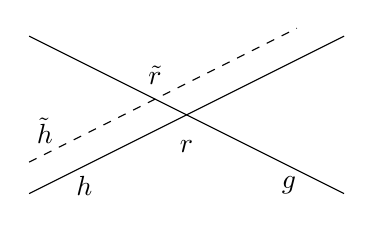
\begin{tikzpicture}[scale =2]
  \draw (-1,-0.5) -- (1,0.5);
  \draw (-1,0.5) -- (1,-0.5);
  \draw[dashed] (-1,-0.3) -- (0.7,0.55);
  \node (draw) at (0,-0.2) {$r$};
  \node (draw) at (-0.2,0.25) {$\tilde{r}$};
  \node (draw) at (-0.9,-0.1) {$\tilde{h}$};
  \node (draw) at (0.65,-0.45) {$g$};
  \node (draw) at (-0.65,-0.45) {$h$};
\end{tikzpicture}
\\gut konditioniert
\end{center}
\end{minipage}
\begin{minipage}{.45\textwidth}
\vspace{1em}
\begin{center}
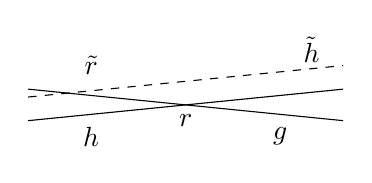
\begin{tikzpicture}[scale =2]
  \draw (-1,-0.1) -- (1,0.1);
  \draw (-1,0.1) -- (1,-0.1);
  \draw[dashed] (-1,0.05) -- (1,0.25);
  \node (draw) at (0,-0.1) {$r$};
  \node (draw) at (-0.6,0.25) {$\tilde{r}$};
  \node (draw) at (0.8,0.35) {$\tilde{h}$};
  \node (draw) at (0.6,-0.2) {$g$};
  \node (draw) at (-0.6,-0.2) {$h$};
\end{tikzpicture}
\\schlecht konditioniert
\end{center}
\end{minipage}

Die Schwierigkeit (Kondition) des Problems hängt vom Winkel ab, in dem sich die Geraden
schneiden:
\begin{itemize}
 \item Stumpfer Winkel: Wird eine Gerade leicht gestört, so erfährt auch
  der Schnittpunkt eine leichte Störung.
 \item Spitzer Winkel: Wir eine Gerade leicht gestört, so ist der Schnittpunkt \emph{stark} gestört.
\end{itemize}
\end{bsp}

\bigskip

Formal: Gegeben ein Eingabewert $x \in X$.
\begin{itemize}
\item $x$ ist nur Repräsentant einer ganzen Menge $E$ von möglichen Eingaben
\item Absolute Fehler:
\begin{equation*}
E = \{ \tilde{x} \in X \; : \; \norm{\tilde{x} - x} \le \delta \}
\end{equation*}
z.B.\ Messfehler
\item Relative Fehler:
\begin{equation*}
E = \{ \tilde{x} \in X \; : \; \norm{\tilde{x} - x} \le \epsilon \norm{x}\}
\end{equation*}
\end{itemize}

Der Lösungsoperator $f$ bildet $E$ auf eine Menge $f(E)$ ab.
\begin{itemize}
\item Die Kondition eines Problems ist das \glqq Verhältnis von $f(E)$ zu $E$\grqq.
\end{itemize}

\bigskip

Quantitativ kann man (fast) nur rechnen, wenn die Fehler klein sind.
Dann kann man eine linearisierte Theorie betreiben.

\medskip

Asymptotische Lipschitz-Bedingung:
\begin{definition}
Die absolute Kondition des Problems $f$ an der Stelle $x$ ist die kleinste Zahl $\kappa_{abs} \ge 0$, so dass
\begin{equation*}
\norm{f(\tilde{x}) - f(x)} \le \kappa_\text{abs} \norm{\tilde{x} - x} + \varphi(\tilde{x})
\end{equation*}
mit $\displaystyle \frac{\varphi(\tilde{x})}{\norm{\tilde{x} - x}} \to 0$ für $\tilde{x} \to x$.
\end{definition}

\begin{itemize}
\item Ist $f$ differenzierbar in $x$, so ist $\kappa_\text{abs} = \norm{f'(x)}$. Dabei ist $f' \in \R^{n \times n}$ die Jacobi-Matrix, $\norm{f'} = \sup_{x \neq 0}\frac{\norm{f'(x)}}{\norm{x}}$ die dazugehörige Matrix-Norm.
\item $f$ heißt \emph{gut konditioniert}, falls $\kappa_\text{abs}$ \glqq klein\grqq{} ist.
\item $f$ heißt \emph{schlecht konditioniert}, falls $\kappa_\text{abs}$ \glqq groß\grqq{} ist.
\end{itemize}

\begin{center}
    \begin{tikzpicture}
    \draw[->] (-1,0) -- (7,0);
    \draw[->] (0,-1) -- (0,4.5);
    \draw (2,0) node[below] {$x$};
    \draw (5,0) node[below] {$x$};
    \foreach \i in {0,1,2,3,4,5}
        {
            \draw (\i + 1, 0.05) -- (\i+1,-0.05);
        }
     \draw plot[smooth] coordinates { (0.1,-0.9) (1,0.1) (2,0.4) (3,0.6) (4,1) (5,2) (6,3.1) (7,4)};
     \draw [decorate,decoration={brace,amplitude=10pt,mirror},xshift=0.4pt,yshift=-0.4pt](1,-0.3) -- (3,-0.3) node[black,midway,yshift=-0.6cm] {\footnotesize $E$};
     \draw [decorate,decoration={brace,amplitude=10pt,mirror},xshift=0.4pt,yshift=-0.4pt](4,-0.3) -- (6,-0.3) node[black,midway,yshift=-0.6cm] {\footnotesize $E$};
     \draw[dashed] (0,0.1) -- (3.5,0.1);
     \draw[dashed] (0,0.6) -- (3.5,0.6);
     \draw [decorate,decoration={brace,amplitude=5pt,mirror},xshift=0.4pt,yshift=-0.4pt](-0.05,0.6) -- (-0.05,0.1) node[black,midway,xshift=-0.6cm] {\footnotesize $f(E)$};
     \draw[dashed] (4,-0.1) -- (4,1.1);
     \draw[dashed] (6,-0.1) -- (6,3.2);
     \draw [decorate,decoration={brace,amplitude=5pt,mirror},xshift=0.4pt,yshift=-0.4pt](6.1,1) -- (6.1,3.1) node[black,midway,xshift=0.6cm] {\footnotesize $f(E)$};
    \end{tikzpicture}
\end{center}
\begin{definition}
Die relative Kondition des Problems $f$ an der Stelle $x$ ist die kleinste Zahl $\kappa_\text{rel} \ge 0$, so dass
\begin{equation*}
\frac{\norm{f(\tilde{x}) - f(x)}}{\norm{f(x)}} \le \kappa_\text{rel} \frac{\norm{\tilde{x} - x} }{\norm{x}}+ \varphi(\tilde{x})
\end{equation*}
mit einem $\varphi$ wie oben.
\end{definition}
Falls $f$ differenzierbar ist, so gilt $\kappa_{rel} = \frac{\norm{x}}{\norm{f(x)}}\norm{f'(x)}$.

\subsection{Kondition von Addition und Subtraktion}

Die Addition zweier Zahlen ist eine Abbildung
\begin{equation*}
f: \R^2 \to \R,
\qquad
f: \begin{pmatrix} a \\ b \end{pmatrix} \mapsto a + b.
\end{equation*}

Als Norm auf $\R^2$ wählen wir die $1$-Norm:
\begin{equation*}
\norm{(a,b)}_1 \colonequals \abs{a} + \abs{b}.
\end{equation*}
Damit ist
\begin{align*}
\norm{f'(a,b)}
 & = \sup_{\substack{x \in \R^2 \\ x \neq 0}} \frac{\norm{f'(a,b) \cdot x}_1}{\norm{x}_1}
   = \sup \frac{\Big\vert (1 \quad 1) \begin{pmatrix} x_1 \\ x_2 \end{pmatrix}\big\vert}{\abs{x_1} + \abs{x_2}} \\
 & =
 \sup \frac{\abs{x_1 + x_2}}{\abs{x_1} + \abs{x_2}} = 1.
\end{align*}
Deshalb:
\begin{equation*}
\kappa_\text{abs} = 1.
\end{equation*}
Relative Kondition:
\begin{equation*}
\kappa_\text{rel}
=
\frac{\norm{(a,b)}_1}{\norm{f(a,b)}} \norm{f'} = \frac{\vert a \vert + \vert b \vert}{\vert a  + b \vert}
\end{equation*}
\begin{itemize}
\item $\kappa_\text{rel} =1 $ falls $a$, $b$ gleiche Vorzeichen haben
\item $\kappa_\text{rel} \gg 1$ falls $a$, $b$ unterschiedliche Vorzeichen haben!
\end{itemize}
Dieses Phänomen heißt \underline{Auslöschung}
\begin{bsp}
$\epsilon = 10^{-7}$
\begin{align*}
a   & = 0{,}123467\hspace{-1.8ex}\overbrace{xxxx}^{\textnormal{unbekannt}} \\
b   & = 0{,}123456xxxx \\
a-b & = 0{,}000011xxxx
\end{align*}
Eingabe: Fehler ab der $7.$ Stelle

Ausgabe: Fehler in der $3.$ Stelle

\medskip

\textbf{Merke:} Subtraktion fast gleicher Zahlen ist zu vermeiden!
\end{bsp}

Auslöschung führt ab und zu zu praktisch relevanten Problemen.

Es gibt diverse Tricks, um Auslöschung zu vermeiden:

\begin{itemize}
  \item Bei derAddition von Zahlenfolgen:

  $\rightarrow$ Sortiere die Zahlenfolge vor der Addition!

  \item Benutze Reihenentwicklung:

  Beispiel: Für kleine $x$ ersetze

 \begin{equation*}
 \frac{1-\cos(x)}{x}
 \qquad \text{durch} \qquad
  \frac{1}{x}\left(1-(1-\frac{x^2}{2} + \frac{x^4}{24} -\dots)\right)
  = \frac{x}{2}\left(1 - \frac{x^2}{12} + \dots\right)
\end{equation*}
\end{itemize}


\subsection{Kondition der Multiplikation}

Die Multiplikation als Abbildung ist
\begin{equation*}
 f : \R^2 \to \R
 \qquad
 f(a, b) = a\cdot b.
\end{equation*}


Ableitung davon:
\begin{equation*}
 f'(a, b) = (b \;\; a)
\end{equation*}

Geeignete Norm: Die $2$-Norm
\begin{equation*}
\norm{(b \;\; a)}_2 \colonequals \sqrt{a^2 + b^2}.
\end{equation*}

Eine dazu passende Matrixnorm: Frobeniusnorm (Ferdinand Georg Frobenius):
\begin{equation*}
\norm{f'(a, b)}_2 = \norm{(b \;\; a)}_2 \colonequals \sqrt{a^2 + b^2}
\end{equation*}

Deshalb:
\begin{align*}
 \kappa_\text{abs}
 & =
 \norm{f'(a, b)}_2 = \sqrt{a^2 + b^2}\\
 %
 \kappa_\text{rel}
 & =
 \frac{\norm{(b \;\; a)}_2}{\abs{f(a, b)}}\norm{f'(a, b)}_2 = \frac{\sqrt{a^2 + b^2}}{\abs{a\cdot b}}\sqrt{b^2 + a^2} = \frac{a^2 + b^2}{\abs{a\cdot b}}.
\end{align*}

Falls $a\approx b$, dann ist
\begin{equation*}
\kappa_\text{rel}\approx \frac{2a^2}{\abs{a^2}} = 2.
\end{equation*}
Die Multiplikation ist dann gut konditioniert.

\bigskip

Sind die Zahlen sehr unterschiedlich, zum Beispiel $a\approx 1$, $b$ sehr klein (oder $a\approx 1$, $b$ sehr groß)
\begin{equation*}
\kappa_\text{rel} = \frac{1+\text{klein}}{\text{klein}} \gg 1.
\end{equation*}

\subsection{Kondition von linearen Gleichungssystemen}

Betrachte das lineare Gleichungssystem
\begin{equation*}
 Ax = b.
\end{equation*}

\paragraph{Der einfache Fall:} Sei $b$ gestört, aber $A$ ohne Fehler bekannt.
\begin{itemize}
\item Lösungsoperator: $f : \R^n \to \R^n$, \qquad $ f(b) = A^{-1}b$
\item Linear

\item Ableitung: $ f'(b) = A^{-1}$

\item Kondition:
   \begin{align*}
    \kappa_\text{abs} &= \norm{f'(b)} = \norm{A^{-1}} \\
    \kappa_\text{rel} &= \frac{\norm{b}}{\norm{f(b)}}\norm{f'(b)} = \frac{\norm{b}}{\norm{A^{-1}b}}\norm{A^{-1}}= \frac{\norm{Ax}}{\norm{x}}\norm{A^{-1}}.
   \end{align*}
\end{itemize}

\paragraph{Weniger einfach:} Sei $b$ ohne Fehler bekannt, aber die Matrix gestört.

Lösungsoperator:
\begin{equation*}
  f : \text{GL}(n) \to \R^n,
  \qquad
  f(A) = A^{-1}b
\end{equation*}
\begin{itemize}
\item nicht linear!
\item Aber differenzierbar. Das folgt z.B.\ aus der Cramerschen Regel.
\end{itemize}

Wir rechnen die Ableitung aus:
\begin{lemma}[\citeauthor{deuflhard_hohmann:1993}, Lemma~2.8]
  Die Abbildung
  \begin{equation*}
   g : \text{GL}(n) \to \text{GL}(n)
   \qquad
   g(A) \colonequals A^{-1}
  \end{equation*}
  ist differenzierbar. Die Richtungsableitung in Richtung $C\in \R^{n\times n}$ ist
\begin{equation*}
\frac{dg(A+tC)}{dt}\bigg|_{t=0} = -A^{-1}CA^{-1}.
\end{equation*}
\end{lemma}

\begin{proof}
\begin{itemize}
  \item Es gilt
   \begin{equation*}
    (A+tC)(A+tC)^{-1} = I, \qquad \forall t\in (-\epsilon,\epsilon).
   \end{equation*}
  \item Differenziere nach $t$:
  \begin{equation*}
   C(A+tC)^{-1} + (A + tC)\frac{d}{dt}(A+tC)^{-1} = 0.
  \end{equation*}
  \item An der Stelle $t = 0$:
   \begin{equation*}
    CA^{-1} + A\frac{d}{dt}(A+tC)^{-1}\bigg|_{t = 0} = 0.
   \end{equation*}
  \item Also
   \begin{equation*}
    \frac{d}{dt}(A+tC)^{-1}\bigg|_{t=0} = -A^{-1}CA^{-1}.
   \qedhere
   \end{equation*}
\end{itemize}
\end{proof}

Die Richtungsableitung ist linear in der Richtung $C$.  Wir schreiben deshalb
\begin{equation*}
 g'(A) C \colonequals -A^{-1}CA^{-1}.
\end{equation*}


\bigskip

Für den Lösungsoperator $f:A \mapsto A^{-1}b$ gilt also
\begin{equation*}
 f'(A)C = -A^{-1}CA^{-1}b = -A^{-1}Cx,
 \qquad
 \forall C\in\R^{n\times n},
\end{equation*}
und ($f'(A)$ ist eine Abbildung $\R^{n\times n}\rightarrow \R^{n\times n}$)
\begin{align*}
 \norm{f'(A)}
 &=
 \sup_{C\neq 0}\frac{\norm{f'(A)C}}{\norm{C}} = \sup_{\norm{C}=1}\norm{f'(A)C}\\
 &=
 \sup_{\norm{C}=1}\norm{A^{-1}Cx} \leq \sup_{\norm{C} =1}\norm{A^{-1}}\norm{C}\norm{x}\\
 &=
 \norm{A^{-1}}\norm{x}.
\end{align*}

Also:
\begin{equation*}
\kappa_\text{abs} = \norm{A^{-1}}\norm{x}
\end{equation*}
und
\begin{equation*}
\kappa_\text{rel} = \frac{\norm{A}}{\norm{x}}\norm{f'(A)}\leq \norm{A}\norm{A^{-1}}.
\end{equation*}

\begin{defi}
  Die Zahl $\kappa(A) \colonequals \norm{A}\norm{A^{-1}}$ (auch: $\operatorname{cond}(A)$) heißt Kondition der Matrix~$A$.
\end{defi}

\begin{itemize}
  \item Bestimmt die Verstärkung von relativen Fehlern in $A$. 
  \item Bestimmt auch die relative Verstärkung von Fehlern in $b$!

  Erinnerung: mit $f:b\mapsto A^{-1}b$ war
  \begin{equation*}
   \kappa_\text{rel}
   =
   \frac{\norm{Ax}}{\norm{x}}\norm{A^{-1}}
   \leq \frac{\norm{A}\norm{x}}{\norm{x}}\norm{A^{-1}}
   =
   \kappa(A).
  \end{equation*}
  \item Beeinflusst die Konvergenzgeschwindigkeit von iterativen Verfahren.
\end{itemize}

Alternative Darstellung:
\begin{equation*}
\kappa(A) \colonequals \frac{\max_{\norm{x}=1}\norm{Ax}}{\min_{\norm{x}=1} \norm{Ax}}\quad \text{(Übung!)}
\end{equation*}

Eigenschaften:
\begin{itemize}
  \item $\kappa(A) \geq 1$.
  \item $\kappa(\alpha A) = \kappa(A), \quad \forall \alpha \in \R, \alpha \neq 0.$
  \item $A$ ist singulär genau dann wenn $\kappa(A) = \infty$.
  \item Falls A symmetrisch ist und $\norm{\cdot} = \norm{\cdot}_2$:
\[\kappa(A) = \frac{\vert \text{betragsmäßig größter Eigenwert}\vert}{\vert\text{betragsmäßig kleinster Eigenwert}\vert}\]
\end{itemize}


\section{Stabilität}

Ein Algorithmus heißt numerisch instabil, wenn es Eingabedaten gibt, bei denen sich
die Rundungsfehler während der Rechnung so akkumulieren, dass ein völlig verfälschtes Ergebnis entsteht.

\begin{bsp}
Werte die Funktion $f(x) = \ln(x - \sqrt{x^2-1})$ an der Stelle $x = 30 $ aus.

\medskip

Tatsächliches Ergebnis:  $f(30) = -4{,}094066\dots$

\begin{itemize}
  \item Kondition des Problems:
   \begin{align*}
    \kappa_\text{abs} = \abs{f'(x)}
    &=
    \bigg|\frac{1}{x-\sqrt{x^2-1}}\left(1-\frac{x}{\sqrt{x^2-1}}\right)\bigg| \\
    %
    &=
    \bigg| \frac{1}{x-\sqrt{x^2-1}} \cdot \frac{\sqrt{x^2-1}-x}{\sqrt{x^2-1}}\bigg|
    = \bigg| \frac{-1}{\sqrt{x^2-1}} \bigg|.
   \end{align*}
  \item An der Stelle $x = 30$:
    \begin{equation*}
     \kappa_\text{abs} = \abs{f'(30)} \approx 0{,}033
    \end{equation*}
    Problem ist gut konditioniert!

  \item Sei der absolute Eingabefehler z.B.\ $\delta = \abs{\hat{x} - x} = 0.05$.

   $\Rightarrow$ Absoluter Ausgabefehler:
   \begin{equation*}
    f(\hat{x}) - f(30) = \abs{f(30 + \delta) - f(30)}\approx \abs{f'(30)}\delta = 0{,}00165.
   \end{equation*}
   Das ist der absolute Ausgabefehler den wir erwarten würden.
\end{itemize}

Wir betrachten, wie ein Algorithmus die Formel auswertet.

\begin{itemize}
  \item Zunächst ist $\sqrt{x^2 - 1}\big|_{x=30} = \sqrt{899} = 29{,}9833287...\approx 30$

   $\Rightarrow$ Bei der Berechnung von $x - \sqrt{x^2 -1}$ kommt es zu Auslöschung.

  \item Angenommen wir rechnen mit $4$ Dezimalstellen:
   \begin{equation*}
    (x - \sqrt{x^2 - 1})\big|_{x=30} = 30 - 29{,}98 = 0{,}02.
   \end{equation*}
  \item Der tatsächliche Wert ist: $30 - 29{,}9833287\ldots = 0{,}0166713\dots$
  \item Absoluter Fehler: $0{,}02 - 0{,}0166713\ldots = 0{,}0033287\ldots$
  \item Der Wert $0{,}02$ wird jetzt in den Logarithmus gesteckt.
  \item Der absolute Fehler wird durch die Kondition des Logarithmus verstärkt:
   \[
    \kappa_{\text{abs}, \text{log}} = \abs{\ln(x)'} = \Big| \frac{1}{x} \Big|.
   \]
   Bei $x = 0{,}02$ ist $\kappa_{\text{abs}, \text{log}} = 50$.
  \item In der Tat ist der Fehler des Gesamtresultats:
   \[
    \abs{f(\hat{x}) - f(30)} = \abs{\ln(0{,}02) - \ln(0{,}0166713\ldots)} = 0{,}1820436\ldots
   \]
  \item Bei einer tatsächlichen Lösung von $-4{,}094066$ is also schon die erste Nachkommastelle falsch!
\end{itemize}
\end{bsp}

\subsection{Modifikation von Algorithmen}

Manchmal können einfache Modifikationen die Stabilität verbessern.

\begin{bsp}
 Löse die quadratische Gleichung
   \[ x^2 - 2px + q = 0.\]
 Lösungsoperator:
   \[f(p, q) = p \pm \sqrt{p^2 - q}.\]
Interpretiere $f$ als Algorithmus:
\begin{itemize}
  \item Problematisch, falls eine Nullstelle nahe bei Null liegt.
  \item Dies ist genau dann der Fall, wenn $q$ sehr klein ist.

   $\Rightarrow \sqrt{p^2 - q}\approx p$, es gibt Auslöschung bei der Subtraktion $p - \sqrt{...}$.
\end{itemize}

Alternative:
\begin{satz}[Satz von Vieta] Seien $x_1$, $x_2$ die Nullstellen von $x^2 - 2px + q$. Dann ist $x_1 x_2 = q$.
\end{satz}
Berechne deshalb $x_1$, $x_2$ durch
\begin{equation*}
 x_1 = p + \operatorname{sgn}(p)\sqrt{p^2 - q},
 \qquad
 x_2 = \frac{q}{x_1}.
\end{equation*}
\end{bsp}

\subsection{Vorwärtsanalyse der Stabilität}

Zur detaillierten Untersuchung der Stabilität eines Algorithmus
fasst man diesen als Kette von elementaren Operationen auf.


\begin{itemize}
  \item Für das Beispiel oben:
  \begin{enumerate}
  \item $g_1 : \R \to \R^2,  \qquad x \mapsto (x,x^2)$
  \item $g_2 : \R^2 \to \R^2, \qquad (y,z) \mapsto (y, z-1)$
  \item $g_3 : \R^2 \to \R^2, \qquad (s,t) \mapsto (s, \sqrt{t})$
  \item $g_4 : \R^2 \to \R, \qquad (u,v) \mapsto u-v$
  \item $g_5 : \R \to \R, \qquad w \mapsto \ln w$
  \end{enumerate}
Insgesamt also $f(x) = (g_5\circ g_4\circ g_3 \circ g_2 \circ g_1)(x)$.
  \item So eine Darstellung wird natürlich schnell sehr umfangreich.
  \item Deshalb kann man auch größere Blöcke nehmen, z.B.
\begin{enumerate}
  \item $\hat{g_1} : \R \to \R^2, \qquad x \mapsto (x,\sqrt{x^2-1})$
  \item $\hat{g}_2 : \R^2 \to \R, \qquad (u,v) \mapsto u-v$
  \item $\hat{g}_3 : \R \to \R, \qquad w \mapsto \ln w$
\end{enumerate}
\end{itemize}



Sei $f = g_k\circ g_{k-1}\circ \dots \circ g_1$.

\begin{itemize}
  \item Wir untersuchen Stabilität bzgl.\ des absoluten Fehlers.
  \item Seien $x = x^{(0)}$ die Eingabedaten, und \[ x^{(i)} = g_i(x^{(i-1)}) = g_i\circ g_{i-1}\circ \dots \circ g_1(x^{(0)}\] die Zwischenergebnisse.
  \item Die tatsächliche Eingabedaten $\hat{x}^{(0)}$ sind mit einem absoluten Fehler behaftet:
    \[
     \hat{x}^{(0)} = x^{(0)} + \delta^{(0)}
    \]
  \item Statt der Zwischenergebnisse $\hat{x}^{(i)}$ tauchen durch Rundnungsfehler verfälschte Ergebnisse
    \[
     \hat{x}^{(i)} = g_i(\hat{x}^{(i-1)}) + \delta^{(i)}
    \]
    auf.
\end{itemize}

Fehlerverstärkung eines einzelnen Schritts $g_i:\R^{n_{i-1}} \to \R^{n_i}$

\medskip

\qquad$\rightarrow$ Kondition von $g_i$ also $\kappa_i = \norm{g_i'}$.

\begin{itemize}
  \item Jeder Fehler $\delta^{(i)}$ wird durch die Ableitung der folgenden Schritte
   $h_i \colonequals g_k \circ g_{k-1}\circ \dots \circ g_{i+1} $ verstärkt.

  \item Wegen der Kettenregel \[h'_i = (g_k\circ g_{k-1}\circ \dots\circ g_{i+1})' = g'_k\cdot g'_{k-1}\cdot\dots\cdot g_{i+1}'\]
  \item Also Einfluss des i-ten Fehlers auf das Resultat $h_i\delta^{(i)}$.

  Fehler insgesamt:
  \[
   \sum_{i=0}^k h_i'\delta^{(i)}.
  \]
\end{itemize}

Algorithmus ist instabil falls zumindest einige der $h_i \gg f'$ sind.

\subsection{Stabilität der Gauß-Elimination}

\begin{itemize}
 \item Kompliziert; wir geben nur ein paar Ergebnisse.

 \item Gauß-Elimination ohne Pivot-Suche ist NICHT stabil.
\end{itemize}

\subsubsection{Rückwärtsanalyse der Gauß-Elimination mit Pivot-Suche:}

\paragraph{Rückwärtsanalyse:} Sei der \emph{Ausgabefehler} gegeben.

Das gestörte Resultat ist die \emph{exakte} Lösung eines gestörten Problem:
\begin{equation*}
 (A +E) \hat{x} = b
\end{equation*}
(Wir betrachten nur Störung in A)

\bigskip

Ein Verfahren heißt stabil im Sinne der Rückwärtsanalyse, falls $\norm{E}$ klein ist.

\medskip

Für die Fehlermatrix $E$ gilt
\begin{equation*}
 \norm{E}_\infty\leq 3\rho_n n^3\epsilon \norm{A}_\infty.
\end{equation*}

Dabei ist:

\begin{itemize}
\item $\epsilon$ die Maschinengenauigkeit.
\item $\rho_n$ der sog. Wachstumsfaktor
 \[
  \rho_n \colonequals \frac{\max_{i,j,k}\abs{a^{(k)}_{ij}}}{\max_{i,j}\abs{a_{ij}}}.
 \]

\end{itemize}


\paragraph{Der Wachstumsfaktor}

Der Wachstumsfaktor ist die für die Stabilität relevante Größe.

Wie verhält sich also $\rho_n$ ?
\begin{itemize}
  \item Falls $A$ strikt diagonal dominant: $\rho_n\leq 2$.
 \item Falls $A$ sym. pos. def. $\rho_n\leq 1$.
\end{itemize}


Allgemein: Für Gauß-Elimination mit Spalten-Pivotsuche: $\rho_n\leq 2^{n-1}$.

\bigskip

Diese Abschätzung ist scharf, denn:
\begin{align*}
A & = \begin{pmatrix}
1& 0& 0& 0& 1\\
-1& 1& 0& 0 &1\\
-1& -1& 1& 0&1 \\
-1& -1& -1&1&1\\
-1&-1&-1&-1&1
\end{pmatrix}\\
%
A^{(2)}
& = \begin{pmatrix}
1& 0& 0& 0& 1\\
0& 1& 0& 0 &2\\
0& -1& 1& 0&2 \\
0& -1& -1&1&2\\
0&-1&-1&-1&2
\end{pmatrix}\\
%
A^{(3)}
& = \begin{pmatrix}
1& 0& 0& 0& 1\\
0& 1& 0& 0 &2\\
0& 0& 1& 0&4 \\
0& 0& -1&1&4\\
0&0&-1&-1&4
\end{pmatrix}\\
%
A^{(4)} & =
\begin{pmatrix}
1& 0& 0& 0& 1\\
0& 1& 0& 0 &2\\
0& 0& 1& 0&4 \\
0& 0& 0&1&8\\
0&0&0&-1&8
\end{pmatrix}
\end{align*}
etc., also
\begin{equation*}
 \rho_h = \frac{\max \abs{a^{(5)}_{ij}}}{\max \abs{a_{ij}}} = 16.
\end{equation*}

Statistisch sieht man $\rho_n \approx n^{\frac{2}{3}}$.

